\documentclass[11pt, a4 paper]{article}
%%---------------------------------------------------
%%  Loading all the packages
%%---------------------------------------------------
\usepackage[utf8]{inputenc}
\usepackage{amsmath,amssymb}
\usepackage[english]{babel}
\usepackage[a4paper, total={6in, 8in}]{geometry}
\usepackage{graphicx}
\usepackage{wrapfig}
\usepackage{booktabs}
\usepackage{wrapfig}
\usepackage{multirow}
\usepackage{csquotes}
\usepackage{multicol}
\usepackage{url}
\usepackage{hhline}
\usepackage{graphicx}
\usepackage{cancel}
\usepackage{tabularx}
\usepackage[font={small,it}]{caption}
\usepackage{listings}
\usepackage{scalerel}
\usepackage{calligra}
\usepackage{bbold}
\usepackage{lipsum}
\DeclareMathAlphabet{\mathcalligra}{T1}{calligra}{m}{n}
\usepackage{float}
\usepackage{amsfonts}
\usepackage{xcolor}
\usepackage{lastpage}
\DeclareMathOperator{\arcsinh}{arcsinh}
\DeclareMathOperator{\arctanh}{arctanh}
\usepackage{physics}
\usepackage{changepage}
%%---------------------------------------------------
%%  Creating the title page
%%---------------------------------------------------
\title{\begin{center}
    
\includegraphics[width=0.1\textwidth]{Pictures/image.jpg}
\end{center}\vspace{1cm}
\textbf{Cracks in the Crystallising Block Universe:\\ A Bayesian Counterargument against common sense. }}
\author{Jan Stevens, \quad r0668263}

%%---------------------------------------------------
%%  Creating the header
%%---------------------------------------------------
\usepackage{fancyhdr}
\pagestyle{fancy}
\fancyhf{}
\lhead{The Cracks in the Crystallised Block Universe}
\rhead{By Jan Stevens}
\cfoot{Page \thepage \hspace{1pt} of \pageref{LastPage}}
%---------------------------------------------------


\begin{document}
\newgeometry{total={6in, 8in}}
\maketitle
\begin{center}

\end{center}

\tableofcontents
\newpage 
\clearpage

\vspace*{0.1\textheight}
\begin{figure}[ht]
    \centering
    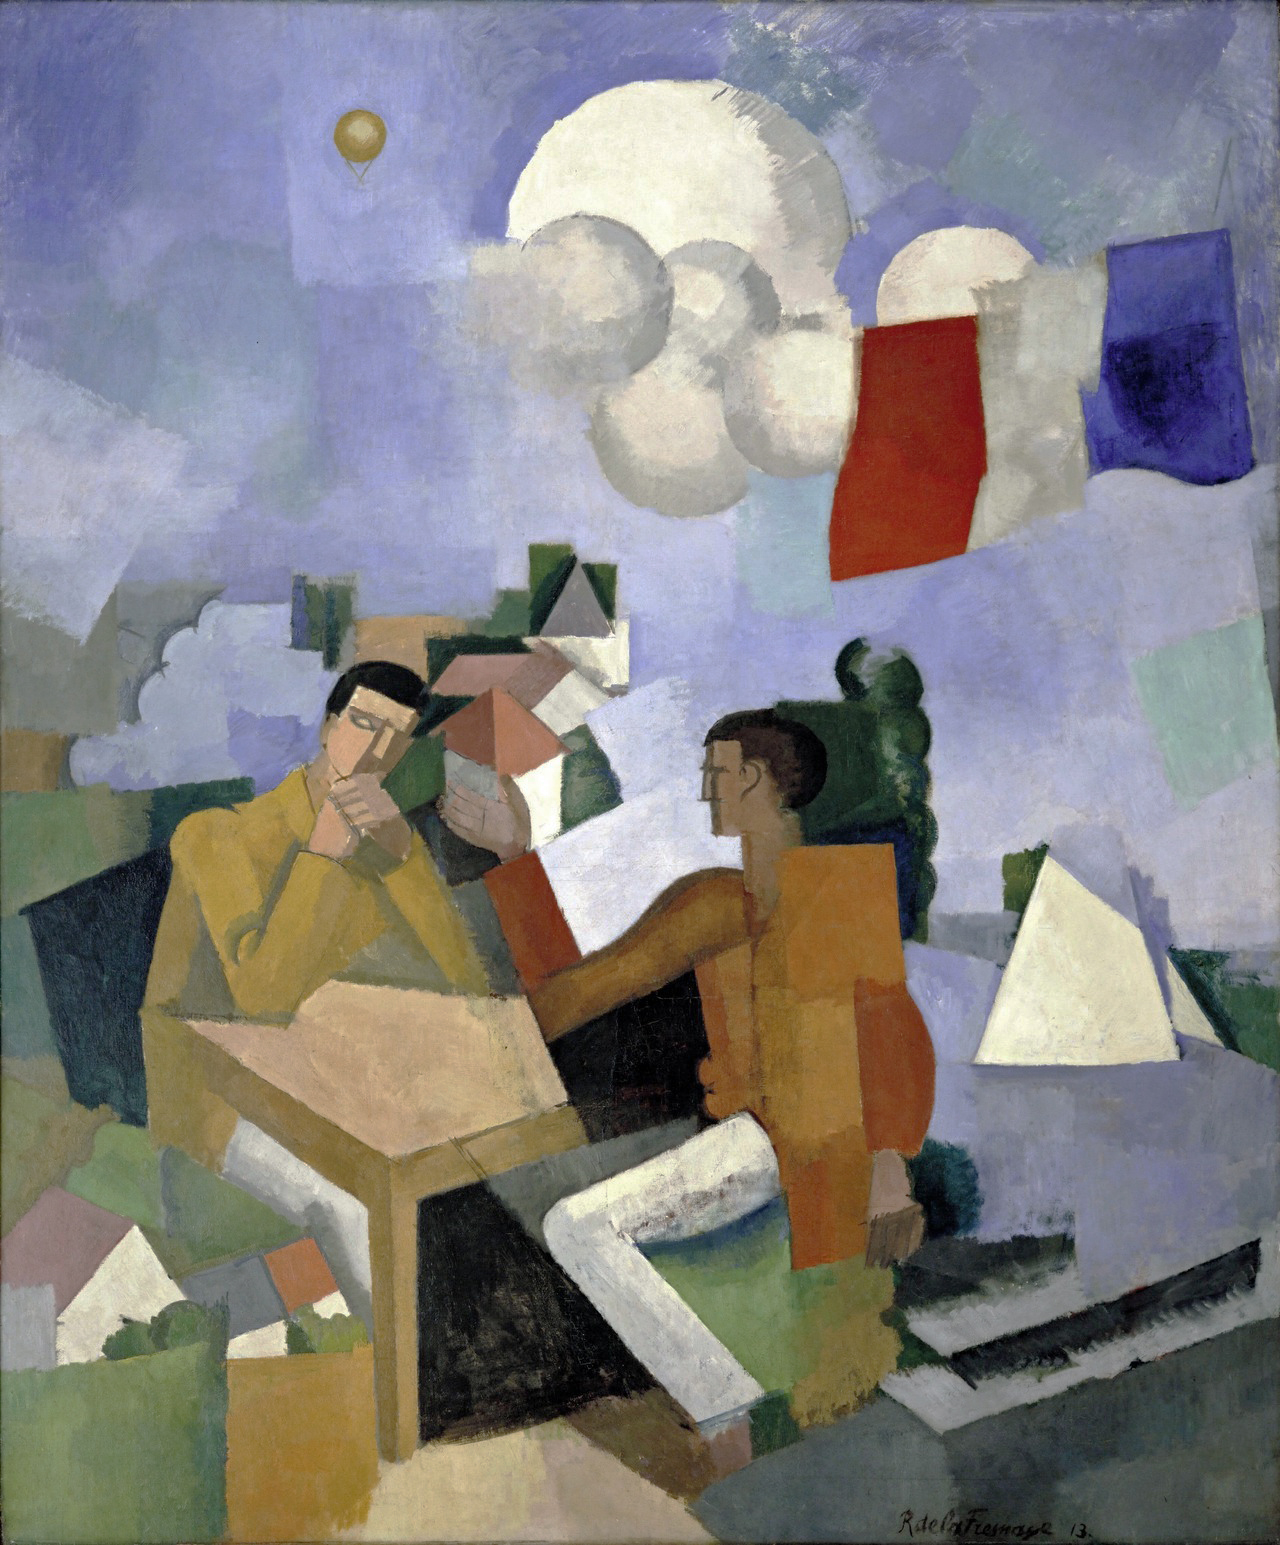
\includegraphics[width=9cm]{Pictures/fresnaye_conquest_of_air.jpg}
    \caption{Roger de La Fresnaye, The Conquest of the Air (1913) \cite{picture}}
    \label{fig:robert}
\end{figure}
\vspace*{0.15\textheight}

\noindent\enquote{\itshape 
We may be in the Universe as dogs and cats are in our libraries, seeing the books and hearing the conversation, but having no inkling of the
meaning of it all.}\bigbreak
\hfill ― William James \cite{quote}\newline

\newpage
\restoregeometry


\section{Introduction}
\begin{multicols}{2}
Every day we all run around looking at our wrists or phones, guided by those rotating arms whilst relentlessly hopping to the next second, minute, hour. Everyone recognises the feeling that time is running and never waiting, but what exactly is that time we are always so focused on. This is not a revolutionary question. There are records of philosophers having this discussion that date back all the way to ancient Egypt.\cite{egypt} The discussions on the nature of time are thus not being resolved any time soon. Nevertheless, thanks to modern physics new light has been shed on some of the central topics in these debates. \\
The General theory of relativity tells us for example that we should not discuss time as a stand alone entity on it's own, but rather conjoint it with our notion of space. The subject of the discussion therefore has shifted to the nature of Space-time itself. Quantum mechanics is another example of a physical theory that drastically changed our view on the universe. From this new mathematical framework of interactions, many apparent paradoxes seem to have followed, often referred to as quantum strangeness. Our view on time has not been spared from this quantum strangeness. Delayed-choice quantum eraser experiments seem to imply that we need to rethink our notion of the `now'.\\
A first step in understanding the space-time we live in is trying to compose a model that fits our experiences. A straight forward mode of operation is looking at our laws of physics, that have been empirically constructed, and build a geometric model best fitting these laws. One of the most well known models that is constructed this way is called ``the Block universe''. The block universe was first proposed by William James in his work ``A Pluralistic Universe'' \cite{quote}.\\
This model is graphically represented in figure \ref{fig:1}. Mathematically speaking, it constructs a fourth time-dimension perpendicular to our three classical space-dimensions while keeping time and space on equal footing.
\begin{wrapfigure}{r}{0.5\linewidth}
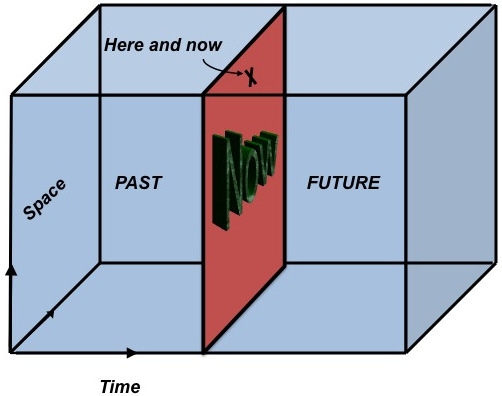
\includegraphics[width=\linewidth]{block.jpeg}
\caption{Block Universe \cite{picblock}}
\label{fig:1}
\end{wrapfigure}
In a more phenomenological way, the model is constructed by taking equal time snippets of our three dimensional space. These are organised in consecutive order so that we can move from slice to slice, and trace out our world line in a four dimensional space-time.\\  Over the years it has gained a lot of popularity, since being viewed as the "common sense" way of interpreting a classical space-time.\\
When modern physics advanced past the Newtonian formalism, some characteristics of the block universe were not consistent anymore with the new empirical evidence. Physical theories, like quantum mechanics and General relativity, imposed some necessary modifications on the Block universe. These revisions still propose a compelling and elegant geometric model of our universe, but the question remains if the tension between this classical model and modern physics is really lifted. I will plead the case, that there is no cut and dry answer to this, since taking modern physics seriously may force us to rethink our entire framework of reality. 
\end{multicols}

\section{Crystallising Block Universe}
\begin{multicols}{2}
We already introduced the Block Universe as the common-sense world view derived from Newtonian mechanics. Due to the nature of the equations of motion in this physical system there is no real difference between the past and future. It could be interpreted as if all apparent motion of the universe is frozen and the only real notion of time is the temporal separation between two events.\\
This temporal indifference breaks down when we look at quantum mechanics. In the Orthodox quantum mechanical interpretation the state of the universe is encoded in a wave function, $\Psi$, defined on it's configuration space. When we perform an experiment, this wave function gives us the probabilities for certain measurement outcomes. This mechanism is called ``the Born rule'' and for a measurement outcome A, it is given by
\begin{equation}
    p(a | \Psi) = |\bra{a} \ket{\Psi}|^2.
\end{equation}
The Born rule tells us that we can not indefinitely predict the outcome of a measurement before the experiment has taken place. It is apparent that, in this classical quantum theory, the moment of the measurement is a non-trivial event. At the moment of measurement the wave function collapses and all the future possibilities reduce to one reality. This sharply contrasts the Block universe in which the apparent now has equal relevance as any other moment in time. Not everything is lost however.\\
The  Block Universe is adapted to take this non-trivial present into account. The resulting model is called the "Growing Block Universe"\cite{dainton}. In this revised model, the hypersurface representing the present is moving towards an undetermined future and the past is still completely disclosed. This model is presented in figure \ref{fig:2}\\
\begin{wrapfigure}{r}{0.4\linewidth}
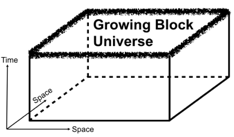
\includegraphics[width=\linewidth]{growing_block.png}
\caption{Growing Block Universe \cite{picgrow}}
\label{fig:2}
\end{wrapfigure}
Furthermore observations like the delayed-choice quantum eraser experiments also need to be taken into account. These types of experiments can be seen as a complex version of Young's double slit experiment. Young found that when a beam of photons passes through two slits and isn't measured, the photons behave like waves. This means that when they hit a back plate instead of the classical dot pattern they will form a interference pattern. Only if someone observes these photons before they pass through the slits, they change their minds and behave as if they were classical particles.\\
The delayed-choice quantum eraser experiment differs from Young's double slit experiments by observing the photons after they already passed through the slits.

\begin{wrapfigure}{l}{0.4\linewidth}
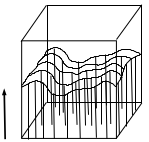
\includegraphics[width=\linewidth]{crystal.png}
\caption{Crystallising Block Universe \cite{crystal}}
\label{fig:3}
\end{wrapfigure}
This alters the way they passed through the slits in the past. It seems like the photons change the way they passed through the double slits in the moments before they notice being watched. Really strange is, that when we delete the information about the photons before they hit the back plate, they again behave like a wave and create an interference pattern.\\
These kind of experiments suggest that we do not live on a hypersurface, that moves uniformly towards the future. Not all the spatial locations move with the same speed towards the future. Some locations seem to be kept back due to quantum uncertainty. The speed at which they propagate in the temporal direction is much lower then their surroundings. Eventually all these events will "crystallize" as the wave function collapses and the static past of our Growing Block Universe is restored.\\
We also need to take relativistic corrections to the Growing Block Universe into account. What changes in this aspect is, that not every point uniformly moves in the temporal direction. In contrary to the crystallising behaviour due to quantum mechanics, general relativity induces only small deformations on our hypersurface. The result is a ``Crystallising Block Universe''\cite{crystal} that much resembles our Growing Block Universe. The difference is that the hypersurface seems a little scarred. The model is represented in figure \ref{fig:3}.
\end{multicols}
\section{Quantum uncertainty}
\begin{multicols}{2}
In the previous chapter we introduced the Crystallising Block Universe, which aims to give a description of space-time consistent based on our modern understanding of physics. It differs from earlier versions by incorporating all of the temporal quantum strangeness currently known in the orthodox quantum theory. This orthodox quantum theory is often referred to as the Copenhagen interpretation. The development of this first quantum mechanical theory was a large collaboration between the great physicists from the 20th century. Especially Niels Bohr, Werner Heisenberg and Max Born are often viewed as the founding fathers of this theory. Eventually it was completed at the fifth Solvay conference\cite{history}. As end result they had a tool by which one could predict the outcome of quantum experiments to a very high degree of precision.\\
Until recently, that is all quantum mechanics really was, a tool to calculate and predict quantum interactions. No consensus was reached on what this new physics implied for the structure of our universe. It is due to this unresolved problem that we need to be cautious when looking the Crystallising Block Universe. It claims to incorporate quantum strangeness into the classical Block Universe, but how can we be sure of this, when the essence of the quantum theory is continuously being doubted.\\
The debate on what the quantum theory tells us about the universe started during the later part of the 20th century. A new generation of ambitious physicists step to the table and tried to resolve the quantum uncertainty surrounding our worldview. Driven by the higher computational power they had at their disposal and disgruntlement towards the 'shut up and calculate' approach of the past, they set out to find a complete and satisfying quantum theory for our universe. Scientists started by delving up the quantum interpretations, that were disregarded during the earlier development of the classical theory. Examples of theories that were revisited and refined are the ``many-worlds interpretation'' by Hugh Everett and the ``pilot wave theory'' by David Bohm. Besides these preexisting interpretations, other more exotic theories were developed with the aim to put the quantum strangeness in an entirely new light. A recent example is ``Quantum Bayesianism'' or  ``Qbism'' developed by Christian Fuchs and Ruediger Schack\cite{Qbism1}\cite{Qbism2}\cite{Qbism3}.\\
All these interpretations differ by how they interpret the wave function. This idea was recently proposed by Ad\´{a}n Cabello\cite{classific}, who further used it to classify all major quantum theories in two distinct groups. The first group proposes a intrinsic realism, by which is implied that the wave function and thus the probabilities connected to an experiment are intrinsic to the system. There are two sub classifications of this intrinsic realism namely: the $\psi$-ontic interpretations and the $\psi$-Epistemic interpretations. A $\psi$-ontic interpretation views the quantum state as a entirely physical aspect of the system. Therefore, the wave function is a real measurable entity in our universe. Under this classification fall the pilot-wave and many-world theory, they promote the wave function to a real substance of reality. Contrastingly,the $\psi$-Epistemic view point reduces the quantum state to an abstract representation of the observer's knowledge of the underlying objective reality. They believe that the wave function directly tells us something about reality and the uncertainty only arises from the fact that the theory is incomplete. One of the famous supporters of this theory was Albert Einstein, who summarised his view on quantum mechanics by:
\begin{quote}
    ``God does not play dice with the universe.''\newline
    ― Albert Einstein  \cite{dice}
\end{quote}
The second group identified by Cabello proposes, a participatory realism  which implies the observer playing a more central role in the quantum theory. This group also consists of two sub classifications: a $\psi$-epistemic and $\psi$-doxastic view point. Most theories in this second group fall under the $\psi$-epistemic approach. In these theories the quantum state represents a degree of knowledge that the observer has about the possible states of the future. It fundamentally differs from intrinsic realism since in these theories quantum mechanics is not seen as a fundamental physical theory. Quantum mechanics is seen as a way of predicting the future state of the universe, but does not say something about the mechanics of the underlying reality. The Orthodox interpretation of quantum mechanics falls under this classification, where the Born rule is used to express the degree of uncertainty surrounding the observer. The $\psi$-doxastic view on quantum mechanics is a more exotic view, where the quantum state expresses the degree of belief the observer has in the possible futures of the system. This kind of interpretation is often called a pragmatic quantum theory.\\
A consequence of this new stance in respect to the quantum world, is that the implications of this theory on our classical world view is entirely different from the orthodox quantum theory. What should be noted is that these participatory realist approaches on quantum mechanics do not deny the existence of an objective world. All they do is acknowledge the fact that quantum mechanics does not deal with this underlying reality. In their eyes quantum mechanics is only concerned with describing and predicting the possible experiences an observer can have in the future. In the next chapter the rather exotic Quantum Bayesian interpretation will be discussed, since this theory  proposes a drastic change in the way we, as observers, interact with the quantum universe.
\end{multicols}
\begin{figure}[h!]
    \centering
    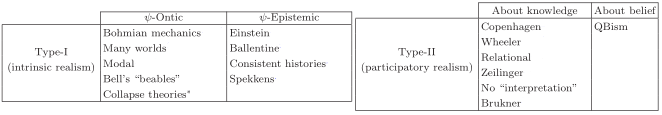
\includegraphics[scale=0.85]{psi.png}
    \caption{Classification of quantum interpretations\cite{classific}}
    \label{fig:my_label}
\end{figure}

\section{Quantum Bayesianism}
\begin{multicols}{2}
Probability is the key difference between classical and quantum theories. Before the first quantum theory was formulated, physicists believed that the world was deterministic. Given enough computational power and exact initial conditions, it seemed possible to exactly calculate the evolution of the entire system.\\
This changed when the classical quantum theory was formulated. The best a physicist could do now was assigning a probability to every possible future state of the system. Consider an experiment where the spin of an electron is measured. Using his quantum knowledge, a physicist calculates that this experiment has an equal probability to measure an up or down spin state. But what is exactly meant, when the physicist assigns a probability of $0.5$ to the spin up state. An orthodox quantum physicist, like Bohr, would use a frequentist definition of probability\cite{prob}. What is meant by this is that if the exact experiment is reproduced and performed many times, the fraction of spin up measurements is exactly half of the total experiments performed. The  frequentist definition of probability is often used by bookkeepers and in most scientific circles.\\
However, a Qbist however would disagree with this kind of interpretation of probability. Inspired by paradoxes in the field of quantum information theory, Qbism adopts a subjective or Bayesian interpretation of probability. The probabilities an agent assigns to certain measurements outcomes are personal reflections of his belief about the quantum system. The only ``rule'' this agent needs to follow is, that he should be rational or in other words dutch book coherent. Dutch book coherence is often explained by considering simple betting games. It boils down to the fact that an agent should not participate in a betting game he is guaranteed to lose. This kind of setup is called a dutch book. What this means for Qbism is that an agent should not assign random probabilities to the possible outcomes, but guarantee rational consistency. From this follows that the Born rule from classical quantum mechanics is not a rule of nature any more, but is reduced to a guideline an agent should follow to assign his probabilities for the future.\\
This is why in Qbism one does not speak of an observer any more, but passive observers are replaced by agents that interact with the universe by observing and assigning their personal probabilities. This is what David Mermin means with his famous quote
\begin{quote}
    ``QBism puts the scientist back into science'' \newline― David Mermin \cite{mermin}
\end{quote}
Using this interpretation of probability, Qbism claims to resolve almost all of the quantum strangeness connected to classical quantum mechanics. A good example is the EPR paradox \cite{EPR}. Imagine entangling two electrons and sending them to the opposite edges of the universe. The paradox arises from the fact that in a classical quantum formulation, when we would measure the spin of one of these, we gain immediate information about the state of the other electron. This violates the locality principle of General relativity, since no information should travel faster than light. A Qbist avoids this problem by understanding, that the only thing that this measurement does, is update the probabilities he would assign for the future. When the agent tries to measure the spin state of the other electron, the only possible dutch book coherent probability he can assign is a probability of 1 to measuring the complementary spin state. If the agent does not do this, he violates his own dutch book coherence, the central rule of Bayesian probability. There is no violation of locality in this quantum theory, since unperformed experiments have no outcomes.\\
The wave function in this theory takes the role of a representation of the belief of an agent with respect to certain possible futures. This makes that the moment of measurement, or collapse of the wave function, gets promoted to a moment of realisation. When the wave function collapses, the agent enforces his probabilities on the universe, resulting in a complex agent-universe dynamic.
\end{multicols}

\section{Where the Block Breaks}
The Qbist interpretation of quantum mechanics illustrates very well the fact that the crystallising block universe may not be the end of the story for the block universe. To really take the quantum mechanical theory and the ongoing development seriously, we should acknowledge these more when creating a consistent block universe.\\
For example, a Qbist style interpretation makes us disregard large scale quantum interactions, since every agent lives in his own local ``reality''. This is due to the fact that the personal probabilities assigned by the agent only incorporate locally relevant phenomena. A larger knowledge of the universe can only be established by rational interactions between multiple agents.\\
In my opinion, exploration of possible space-time interpretations consistent with modern quantum theory is necessary, however a healthy amount of reticence is needed in order to not overestimate newly established models.
\begin{multicols}{2}
\end{multicols}

\newpage
\begin{thebibliography}{}
\bibitem{picture}
R. de La Fresnaye (1913). “The Conquest of the Air''.  accessed on 27/12/2019 from \url{https://www.moma.org/collection/works/79181}
\bibitem{quote}
W. James (1977). ``A Pluralistic Universe''. p.140. Harvard University Press
\bibitem{egypt}
J. Barlett (2014). ``Bartlett's Familiar Quotations''
\bibitem{picblock}
Taken from \url{http://thehumblefuturist.com/retro-causality/} on 09/01/2020
\bibitem{dainton}
B. Dainton (2010). ``Time and Space''. Acumen
\bibitem{picgrow}
Taken from \url{https://www.quora.com/Which-has-more-support-in-relativity-the-block-universe-theory-or-the-growing-block-universe-theory} on 09/01/2020
\bibitem{crystal}
G. Ellis, T. Rothman (2018). ``Spacetime: The Crystallizing Block Universe''
\bibitem{history}
G. Bacciagaluppi, A Valentini (2009). ``Quantum Theory at the Crossroads: Reconsidering the 1927 Solvay Conference''
\bibitem{Qbism1}
C. A. Fuchs (2010). ``QBism, the Perimeter of Quantum Bayesianism''
\bibitem{Qbism2}
C. A. Fuchs, R. Schack (2013). “Quantum-Bayesian Coherence: The No-Nonsense Version''
\bibitem{Qbism3}
C. A. Fuchs, D. Mermin, R. Schack (2013). ``An Introduction to QBism
\bibitem{classific}
A. Cabello (2016). ``Interpretations of quantum theory: A map of madness''
\bibitem{dice}
A. Einstein, M. Born (1971). ``The Born-Einstein letters''. publisher: Macmillan
\bibitem{mermin}
D. Mermin (2014). ``QBism puts the scientist back into science''. Nature
\bibitem{prob}
Hájek, Alan (2019). ``Interpretations of Probability'', The Stanford Encyclopedia of Philosophy 
\bibitem{EPR}
A. Einstein, B. Podolsky, N. Rosen (1935). ``Can Quantum-Mechanical Description of Physical Reality be Considered Complete?''. Physical Review. 47
with an Application to the Locality of Quantum Mechanics''
\bibitem{Qbism5}
C. Fuchs (2015). ``My Struggles with the Block Universe''
\bibitem{Qbism6}
D. Mermin (2018). ``Making Better Sense of Quantum Mechanics''
\bibitem{Book}
H. C. Baeyer (2016). ``Qbism, The Future of Quantum Physics'' Harvard University press
\bibitem{bayesianism}
Healey, Richard (2017). ``Quantum-Bayesian and Pragmatist Views of Quantum Theory'', The Stanford Encyclopedia of Philosophy 
\end{thebibliography}
\end{document}